\documentclass[a4paper]{article}
\usepackage[a4paper,pdftex]{geometry}
\usepackage[english]{babel}
\usepackage{amsmath,amsfonts}
\usepackage[pdftex]{graphicx}
\usepackage{epstopdf}
\usepackage{fancyhdr}
\usepackage{lastpage}
\usepackage{setspace}
\usepackage{xcolor}
\usepackage{hyperref}
\usepackage{url}
\usepackage[all]{xy}
\usepackage[toc,page]{appendix}
\usepackage[T1]{fontenc}   

% Page style
\pagestyle{fancy}

% Page numbering
\lhead{}
\cfoot{}
\rfoot{\thepage}

\author{Chiel Kooijman\\5743028\\\url{Chiel999@gmail.com} \and
Steven Laan\\6036031\\\url{S.Laan@uva.nl} \and
Camiel Verschoor\\10017321\\\url{Verschoor@uva.nl} \and
Auke Wiggers\\6036163\\\url{A.J.Wiggers@uva.nl}}

\title{Collaborative Visual SLAM\\\normalsize Multi-Agent Visual Odometry and SLAM with humanoid robots.\\Project AI (6 EC)\\Artificial Intelligence\\Faculty of Science\\University of Amsterdam}

\begin{document}

%% FRONT PAGE
\thispagestyle{empty}
\begin{center}
\Large\textsc{Collaborative Visual SLAM}\\
\normalsize\textsc{Multi-Agent Visual Odometry and SLAM with humanoid robots.}

\vspace{2cm}

\begin{figure*}[!ht]
\centering
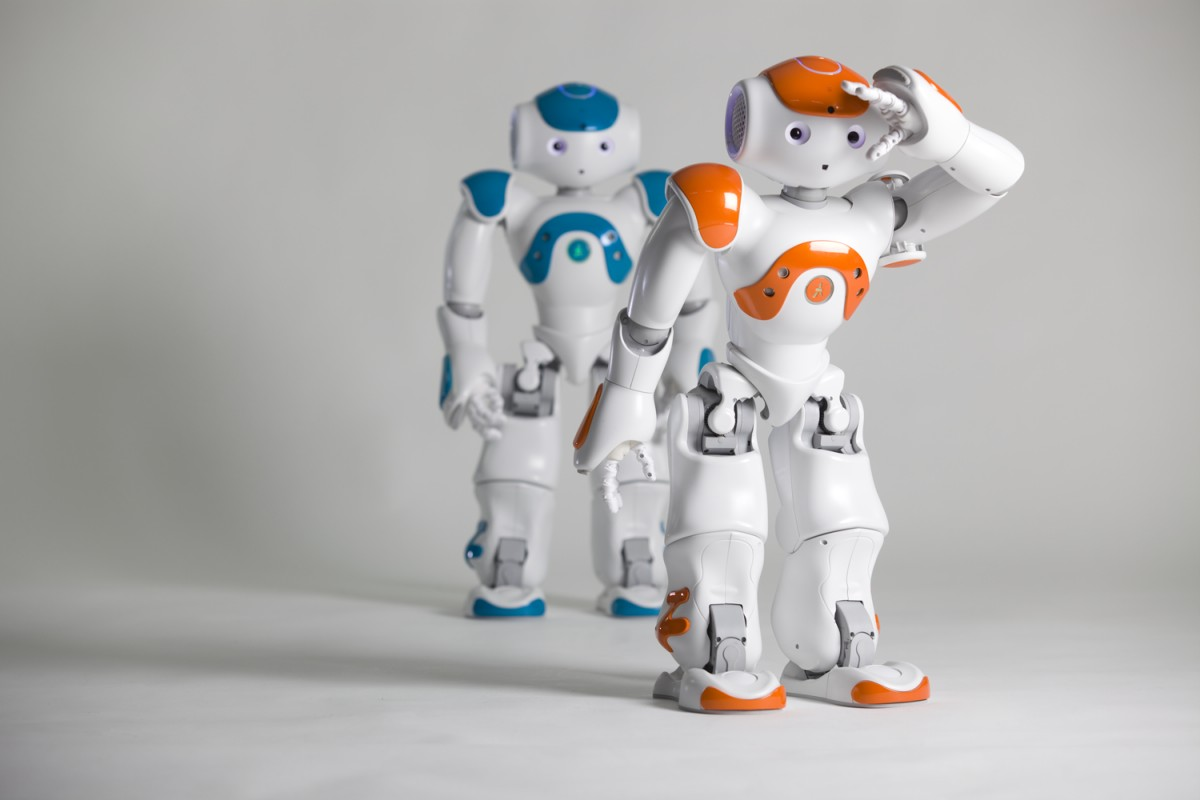
\includegraphics[width=\textwidth]{images/front.jpg}
\end{figure*}

\subsubsection*{A Artificial Intelligence project by Auke J. Wiggers, Camiel R. Verschoor,\\Chiel Kooijman and Steven Laan}
\end{center}

\newpage

% EMPTY PAGE
\thispagestyle{empty}
\mbox{}
\newpage

% OFFICIAL FRONT PAGE
\maketitle
\clearpage

% TABLE OF CONTENTS
\thispagestyle{empty}
\tableofcontents
\clearpage

\section{Introduction}

\section{Related Work}

\section{Theory}

\section{Pipeline}
In this section, the pipeline of our proposed system is described stepwise.

\begin{figure}[!hb]
\centerline{
\xymatrix{
Calibration\ar[rr] & & Feature\ Extraction \ar[rr] & & Feature\ Matching \ar[rr] & & 3D\ map\ reconstruction \ar[rr] 2D\ and\ 3D\ feature\ matching
%User\ar[rr]^{Posts\ message\ on} & & Twitter \ar[dd]^{Message\ is\ extracted\ by}\\
%& &\\
%Recommendation \ar[uu]^{Play\ to} & & System \ar[ll]^{Provides}\\
}
}
\caption{Schematic overview of the pipeline of the system}
\label{fig:system}
\end{figure}

\subsection{Calibration}
\subsection{Feature Extraction}
\subsection{Feature Matching}
\subsection{3D Map reconstruction}
\subsection{2D feature and 3D feature Matching}



\section{Experimental Setup}

\section{Results}

\section{Discussion}

\section{Conclusion}


\end{document}